\documentclass[11pt,a4paper]{report}
\usepackage[portuges]{babel}
\usepackage[utf8]{inputenc}
\usepackage{graphicx}
\usepackage{url}
\usepackage{enumerate} 
\usepackage{lmodern}

%\usepackage{apalike} % gerar biliografia no estilo 'named' (apalike)

\usepackage{color}
\usepackage{multirow} 
\usepackage{array} 
\usepackage[pdftex]{hyperref}
\usepackage[font=small,labelfont=bf]{caption}



\definecolor{saddlebrown}{rgb}{0.55, 0.27, 0.07}

\usepackage{listings}  % para utilizar blocos de texto verbatim no estilo 'listings'
%paramerização mais vulgar dos blocos LISTING - GENERAL
\lstset{
	basicstyle=\small, %o tamanho das fontes que são usadas para o código
	numbers=left, % onde colocar a numeração da linha
	numberstyle=\tiny, %o tamanho das fontes que são usadas para a numeração da linha
	numbersep=5pt, %distancia entre a numeração da linha e o codigo
	breaklines=true, %define quebra automática de linha
    frame=tB,  % caixa a volta do codigo
	mathescape=true, %habilita o modo matemático
	escapeinside={(*@}{@*)} % se escrever isto  aceita tudo o que esta dentro das marcas e nao altera
}
%
\lstset{ 
	language=Python}							% choose the language of the code
%	basicstyle=\ttfamily\footnotesize,		% the size of the fonts that are used for the code
%	keywordstyle=\bfseries,					% set the keyword style
%	%numbers=left,							% where to put the line-numbers
%	numberstyle=\scriptsize,				% the size of the fonts that are used for the line-numbers
%	stepnumber=2,							% the step between two line-numbers. If it's 1 each line
%											% will be numbered
%	numbersep=5pt,							% how far the line-numbers are from the code
%	backgroundcolor=\color{white},			% choose the background color. You must add \usepackage{color}
%	showspaces=false,						% show spaces adding particular underscores
%	showstringspaces=false,					% underline spaces within strings
%	showtabs=false,							% show tabs within strings adding particular underscores
%	frame=none,								% adds a frame around the code
%	%abovecaptionskip=-.8em,
%	%belowcaptionskip=.7em,
%	tabsize=2,								% sets default tabsize to 2 spaces
%	captionpos=b,							% sets the caption-position to bottom
%	breaklines=true,						% sets automatic line breaking
%	breakatwhitespace=false,				% sets if automatic breaks should only happen at whitespace
%	title=\lstname,							% show the filename of files included with \lstinputlisting;
%											% also try caption instead of title
%	escapeinside={\%*}{*)},					% if you want to add a comment within your code
%	morekeywords={*,...}					% if you want to add more keywords to the set
%}

\usepackage{xspace}

\parindent=0pt %espaço a deixar para fazer a  indentação da primeira linha após um parágrafo
\parskip=2pt % espaço entre o parágrafo e o texto anterior

\setlength{\oddsidemargin}{-1cm} %espaço entre o texto e a margem
\setlength{\textwidth}{18cm} %Comprimento do texto na pagina
\setlength{\headsep}{-1cm} %espaço entre o texto e o cabeçalho
\setlength{\textheight}{23cm} %altura do texto na pagina

% comando '\def' usado para definir abreviatura (macros)
% o primeiro argumento é o nome do novo comando e o segundo entre chavetas é o texto original, ou sequência de controle, para que expande
\def\darius{\textsf{Darius}\xspace}
\def\antlr{\texttt{AnTLR}\xspace}
\def\pe{\emph{Publicação Eletrónica}\xspace}
\def\titulo#1{\section{#1}}    %no corpo do documento usa-se na forma '\titulo{MEU TITULO}'
\def\super#1{{\em Supervisor: #1}\\ }
\def\area#1{{\em \'{A}rea: #1}\\[0.2cm]}
\def\resumo{\underline{Resumo}:\\ }

%\input{LPgeneralDefintions} %permite ler de um ficheiro de texto externo mais definições



\title{

\begin{center}

\includegraphics[scale=0.3]{images/um}
\end{center}

Processamento de Linguagens \\
		3º ano de MIEI\\  \vspace{1cm}
       \textbf{Trabalho Prático 2}\\ 
			  \vspace{1cm} Relatório de Desenvolvimento \\
      GIC/GT + Compiladores\\ \vspace{2cm}
\large{Grupo 46}}

\author{ Ana Filipa Pereira\\ (A89589) \and Carolina Santejo\\ (A89500)
         \and Raquel Costa\\ (A89464)
       }

\date{\vspace{2cm}\today} 

\begin{document}


\maketitle % apresentar titulo, autor e data




\begin{abstract}  % resumo do documento
Este primeiro trabalho realizado no âmbito da cadeira de Processamento de Liguagens consistiu na criação de uma linguagem imperativa , à qual demos o nome de \textit{EtelBina} e de um compilador que gerásse pseudo-código \textit{Assembly} para a \textit{Virtual Machine}.
Neste relatório está explicado detalhamente todos os passos da resolução de do projeto, nomeadamente as escolhas feitas para a linguagem desenvolvida e o raciocínio na base das soluções propostas.\par
É de realçar que o desenvolvimento do projeto foi faseado, na medida em que, inicialmente elaborou-se a gramática independente do contexto,passando-se depois, para o analisador léxico. O último passo consistiu no desenvolvimento da gramática tradutora com o objetivo de criar um compilador de linguagens.
\end{abstract}



\tableofcontents 

\listoffigures 




\chapter{Introdução} \label{chap:intro} 			%  -------------------------------------- INTRODUÇÃO --------------------------------------------

\subsection{Enquadramento e Contexto}
\textit{Área: Processamento de Linguagens}\par
\vspace{2ex}
Como já foi referido, neste projeto,foi-nos pedido que desenvolvessemos uma linguagem imperativa simplificada, e, posteriormente um compilador responsável por interpretá-la. \par
Dada a complexidade da programação em \textit{Assembly}, é muito mais fácil e intuitivo escrever linhas de código de uma dada linguagem e ter uma ferramenta que o converta diretamente para código que a máquina seja capaz de interpretar.

\vspace{3ex}
 
 
\subsection{Problema e Objetivo}
Neste segundo trabalho prático da unidade curricular de Processamento de Linguagens, o problema consistiu em desenvolver uma linguagem de programação imperativa simples a nosso gosto, mas que contivesse as seguintes funcionalidades:
\begin{itemize}
	\item Declaração de variáveis do tipo inteiro;
	\item efetuar instruções algorítmicas básicas;
	\item ler do \textit{standard input} e escrever no \textit{standard output};
	\item efetuar instruções condicionais;
	\item efetuar instruções cíclicas, sendo que no nosso caso foi implementado o ciclo \textit{repeat-until};
	\end{itemize}
Posto isto, foi necessário criar um compilador para a nossa linguagem e  que fosse capaz de gerar pseudo-código \textit{Assembly} da \textit{Virtual Machine}.
Os principais objetivos deste projeto, consistiram não só em desenvolver um compilador através da geração de código para a \textit{Virtual Machine}, mas também em aumentar o conhecimento em engenharias de linguagens e em desenvolver processadores de linguagens segundo o método da tradução dirigida pela sintaxe.Além disto, este projeto contribui para o aumento do conhecimento na área da programação generativa.\par 
\vspace{3ex}

\subsection{Estrutura do Relatório}
Este relatório possui 5 capítulos.\par
No capítulo 1, Introdução, é feito o enquadramento e contextualização do projeto, bem como uma breve descriçãoao do problema em mãos. É feita também, uma referência às decisões tomadas no trabalho.\par
No capítulo 2, Análise e Especificação, é feita uma descrição informal do desafio em questão, além de serem especificados os requisitos necessários.
No capítulo 3, Implementação, é explicada , detalhadamente, a resolução do problema, nomeadamente o desenvolvimento da gramática,a parte relativa ao analisador léxico e a parte relativa ao analisador sintático.\par
No capítulo 4, Codificação e Testes, são apresentados testes realizados e os resultados obtidos.\par
No capítulo 5, Conclusão, é feita uma análise geral do projeto.






\chapter{Análise e Especificação} \label{chap:analiseEspecificacao}		% ----------------------- Análise e Especificação ----------------------------------


\subsection{Descrição informal do problema}

Desenvolver uma linguagem de programação e o respetivo compilador. Com recurso a uma gramática tradutora gerar código assembly para ser lido por uma máquina de stack virtual (VM).

\subsection{Especificação dos requisitos}

De forma a responder devidamente ao problema proposto foram definidos inicialmente alguns requisitos a cumprir ao longo da sua elaboração:

\begin{itemize}

\item{Elaborar uma linguagem bem definida}

\item{Efetuar a análise léxica e sintática}

\item{Definir estruturas de dados para guardar informações necessárias}

\item{Elaborar as regras de tradução para assembly}
	
\end{itemize}




\chapter{Concepção/Desenho da Resolução}			% --------------------------------- Concepção/desenho da Resolução ---------------------------------


\section{Gramática Independente de Contexto (GIC)}
O primeiro passo do desenvolvimento deste projeto, consistiu na criação de uma gramática regular independente do contexto que representasse a linguagem imperativa definida pelo grupo.\par
A gramática inicia com o símbolo não terminal \textit{Aplicacao} que deriva em dois símbolos não terminais designados por \textit{Declaracoes} e \textit{Content}. Isto permite dividir o programa em dois grandes blocos: as declarações das variáveis ,sempre no início do programa, e o conteúdo restante.\par
\begin{center}
	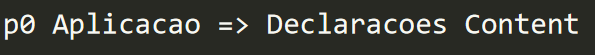
\includegraphics[width=50mm,scale=2]{images/blocos}
	\captionof{figure}{Regra de produção referente à \textbf{Aplicacao}}
\end{center}


\vspace{1ex}
Começemos por explicar as declarações de variáveis.\par
Na nossa linguagem, é permitido que não haja qualquer definição de variáveis. No entanto, se houver, há algumas regras que a ter em conta:
 \begin{itemize}
 	\item No fim de uma declaração coloca-se um ponto;
 	\item Qualquer declaração começa com o tipo da variável a declarar, sendo que neste trabalho só se permite usar o tipo \textit{int};
 	\item Após o tipo da variável, é obrigatório dar-lhe um nome;
 	\item É possível declarar uma variável inteira, um \textit{array} de inteiros ou um \textit{array} bidimensional de inteiros;
 	\item Quando se declara um \textit{array} é obrigatório colocar,após o nome, entre parênteses retos a sua dimensão;
 	\item Quando se declara um \textit{array} bidimensional é obrigatório colocar,após o nome,dois pares seguidos de parênteses retos, sendo que dentro deles se coloca as dimensões do \textit{array};
 	\item É possível fazer atribuições às variáveis.
 	\item Para atribuir um dado valor inteiro a uma variável, coloca-se após o seu nome,  um símbolo "=" e de seguida o valor a númerico desejado;
 	\item Para definir os valores de um array,basta, após o seu nome, colocar um símbolo "=" e entre chavetas colocar os valores desejados separados por vírgulas;
 	\item Para definir os valores de um array,basta, após o seu nome, colocar um símbolo "=" e entre chavetas colocar os valores desejados separados por vírgulas;
 	\item Para definir os valores de um array bidimensional,basta, após o seu nome, colocar um símbolo "=" e entre chavetas colocar listas de números separadas por vírgulas. Cada uma dessas linhas é formada por chavetas,e entre elas, os vários valores númericos separados por vírgula;
 	
 \end{itemize}
\vspace{3ex}
\begin{figure}[hbt!]
	\centering
	\hspace*{-1cm}
	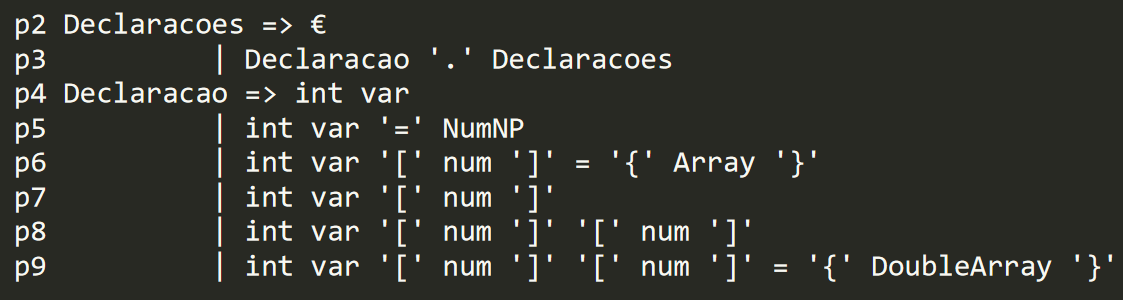
\includegraphics[width=100mm,scale=4]{images/declaracoes}
	\caption{Regras de produção referentes às \textit{Declaracoes}}
\end{figure}

\vspace{0.01ex}
\begin{figure}[hbt!]
	\centering
	\hspace*{-1cm}
	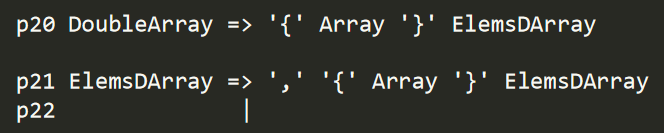
\includegraphics[width=100mm,scale=1]{images/double_Array}
	\caption{Regra de produção referente aos \textit{DoubleArrays}}
\end{figure}
\vspace{3ex}
Passemos agora para a explicação do resto do contéudo do programa.

\vspace{1ex}
\begin{figure}[hbt!]
	\centering
	\hspace*{-1cm}
	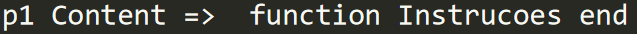
\includegraphics[width=80mm,scale=1]{images/content}
	\caption{Regra de produção referente ao \textit{Content}}
\end{figure}

\vspace{1ex}
Após as declarações das variáveis, é necessário escrever o nome da função (a primeira letra terá de ser minúscula), seguida de parênteses curvos e de dois pontos.Entre os dois pontos não se colocam nada, pois neste trabalho consideramos que as funções não recebem argumentos.Por outro lado, no fim do código deverá ser colocada expressão \textit{end} que simboliza o fim do programa.\par 
Posto isto, temos as instruções a executar.\par
\begin{figure}[hbt!]
	\centering
	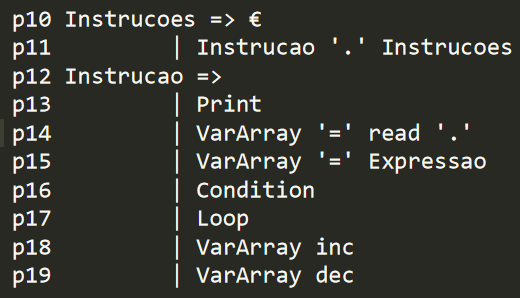
\includegraphics[width=70mm,scale = 1]{images/instrucoes}
	\caption{Regras de produção referentes às instruções do programa}
	\label{fig:instruções}
\end{figure}

 Na nossa linguagem é permitido que não sejam definidas nenhumas instruções, mas caso sejam,todas tem que ter no fim um ponto.
 As instruções que podem ser executadas são:
 
 \begin{itemize}
 	\item Atribuir a uma variável, a uma posição do array ou a uma posição do array bidimensional, um valor lido do \textit{standard input},bastando ,para isso, colocar em frente um "=" e a palavra \textit{read};
    \item Incrementar uma variável, um valor de um array normal ou bidimensional,em uma unidade, bastando para isso, colocar em frente "++" ;
 	\item Decrementar uma variável, um valor de um array normal ou bidimensional,em uma unidade, bastando para isso, colocar em frente "--" ;
 	\item Mostrar no \textit{standard output} o valor de uma variável, ou o valor que se encontra numa dada posição do array normal ou do array bidimensional,;
 	\item Atribuir a uma variável, a uma posição do array ou a uma posição do array bidimensional, o resultado de uma expressão algébrica,bastando ,para isso, colocar em frente um "=" e a respetiva expressão desejada;
 	\item Fazer um ciclo \textit{repeat until}. Após o \textit{repeat}, deverão ser escritas,entre chavetas, as instruções a executar. Depois da última chaveta deve aparecer o \textit{until}, que ,por sua vez, tem à frente, entre parenteses curvos, a condição;
 	\item Utilizar as estruturas de decisão: \textit{if} e \textit{if-else}. Aqui, a condição que se quer verificar, pode ser uma única condição, ou uma composição delas utilizando os operadores lógicos \textit{and} e \textit{or}. Uma condição pode ser uma comparação entre: expressões algébricas, variáveis, ou valores de uma dada posição da matriz ou do array. Essa comparação pode ser de igualdade (\textit{equals}), de menor (<), de maior (>), menor ou igual (\textit{lessEq}) e maior e igual(\textit{moreEq}).É de realçar que nesta linguagem utiliza-se o simbolo "!" quando queremos efetuar a negação de uma expresão lógica.
 	
\end{itemize}
\vspace{2ex}


\begin{figure}[hbt!]
	\centering
	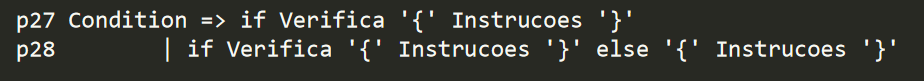
\includegraphics[width=90mm,scale = 2]{images/ifs}
	\caption{Regras de produção referentes às estruturas de decisão}
	\label{fig:instruções}
\end{figure}

\begin{figure}[hbt!]
	\centering
	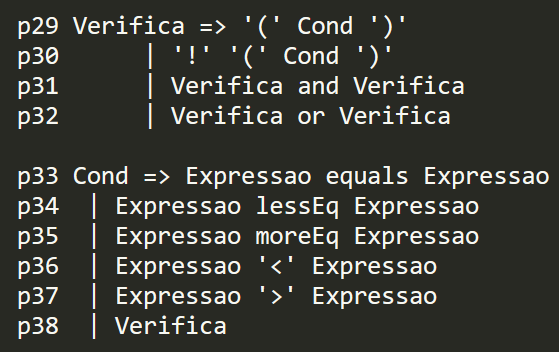
\includegraphics[width=70mm,scale = 1]{images/verifica}
	\caption{Regras de produção referentes às condições}
	\label{fig:instruções}
\end{figure}

\section{Implementação}
\subsection{Analisador Léxico}
Como é possível ver pelo código abaixo, os símbolos terminais representados por parenteses, por ponto e todos aqueles que são relativos a operações lógicas e algébricas, são considerados \textit{literals}. Para todos os outros, foi necessário definir a expressão regular adequada para os identificar. \par
Na situação em que se incrementa um dado valor em uma unidade, apesar do símbolo terminal se chamar \textit{inc}, em termos da linguagem, utiliza-se a expressão "++". O mesmo ocorre para a ação de decrementar,sendo que ,neste caso, utiliza-se a expressão "--".\par
É de realçar que, no caso dos números negativos, o grupo começou por usar a seguinte ER:  r'-\textbackslash d+' 
 No entanto, verificou-se que ocorria um erro, uma vez que o \textit{lexer} não conseguia distinguir o número negativo de uma operação de subtração. Desta forma, a ER foi mudada para r'\textbackslash(-\textbackslash d+\textbackslash)', fazendo com que, na nossa linguagem, os números negativos devams er colocados entre parênteses curvos. Assim, aplicando o conhecimento já usado no primeiro trabalho prático, utiliza-se um \textit{search} e aplica-se o group(0) ao resultado de maneira a obter apenas o número que está entre parênteses. Assim que temos esse valor, este é colocado em \textit{t.value}.


\vspace{3ex}
\begin{verbatim}
tokens = ['and','or', 'lessEq', 'moreEq','equals', 'int', 'print', 'read', 'if',
'else', 'end', 'repeat', 'until', 'num', 'numNeg',
'var', 'string', 'function','inc','dec']

literals = ['*', '+' ,'/', '-', '=', '(', ')', '.', '<', '>', ',', '!', 
            '{', '}', '[', ']']

t_and = r'and'
t_lessEq = r'lessEq'
t_moreEq = r'moreEq'
t_equals = r'equals'
t_inc = r'\+\+'
t_dec = r'--'
t_int = r'int'
t_print = r'print'
t_read = r'read'
t_else = r'else'
t_end = r'end'
t_repeat = r'repeat'
t_until = r'until'


def t_num(t):
r'\d+'
#t.value = int(t.value)
return t

def t_numNeg(t):
r'\(-\d+\)'
res = re.search(r'-\d+', t.value)
t.value = res.group(0)
return t

def t_if(t):
r'if'
return t

def t_or(t):
r'or'
return t

def t_function(t):
r'[a-z]\w+\(\):'
return t

t_string = r'"[^"]+"'
t_var = r'\w+'


t_ignore = " \t\n"

def t_error(t):
print('Illegal character: ', t.value[0])
t.lexer.skip(1)

lexer = lex.lex()

\end{verbatim}

\subsection{Gramática Tradutora (GT)}
\qquad Através do \textit{Yacc} versão \textbf{PLY} do \textit{python} foi criada uma gramática tradutora, a partir da qual foi possível desenvolver um processador de linguagens. Esta teve por base a gramática independente de contexto desenvolvida numa primeira fase do trabalho, ao longo do seu desenvolvimento houveram alguns acertos a fazer dependendo dos resultados que eram necessários obter.\par
\qquad A abordagem adotada no desenvolvimento da gramática foi um parser \textit{bottom-up}, de forma a satisfazer a condição LR().\par
\qquad Posto isto, o seguinte código apresentado retrata o que foi feito inicialmente no ficheiro Yacc, antes do grupo começar a desenvolver uma solução que consiga gerar código para uma máquina de stack virtual, que neste caso a usada é a VM (Virtual Machine).

Em primeiro lugar definimos o axioma \textit{Aplicação} e o símbolo não terminal \textit{Content} :\par
\begin{verbatim}
def p_Aplicacao(p):
    "Aplicacao : Declaracoes Content"
    pass

def p_Content(p):
    "Content : function Instrucoes end"
    pass
\end{verbatim}

De seguida definimos o simbolo \textit{Declaracoes} e cada \textit{Declaracao} existente na grmática elaborada, sendo que no caso dos arrays foi necessário recorrer à criação de novos simbolos que permitissem preencher um array aquando a declaração do mesmo.

\begin{verbatim}
def p_Declaracoes(p):
    " Declaracoes : Declaracao '.' Declaracoes"
    pass

def p_DeclaracoesEmpty(p):
    "Declaracoes : "
    pass

def p_Declaracao(p):
    "Declaracao : int var"
    pass

def p_Declaracao_Array(p):
    "Declaracao : int var '[' num ']'"
    pass

def p_Declaracao_DoubleArray(p):
    "Declaracao : int var '[' num ']' '[' num ']'"
    pass


def p_Declaracao_atribuicao(p):
    "Declaracao : int var '=' NumNP"
    pass

def p_Declaracao_Array_Atribuicao(p):
    "Declaracao : int var '[' num ']' '=' '{' Array '}'"
    pass


def p_Declaracao_DoubleArray_Atribuicao(p):
    "Declaracao : int var '[' num ']' '[' num ']' '=' '{' DoubleArray '}'"
    pass


def p_DoubleArray(p):
    "DoubleArray : '{' Array '}' ElemsDArray"
    pass

def p_ElemsDArray(p):
    "ElemsDArray : ',' '{' Array '}' ElemsDArray "
    pass

def p_ElemsDArrayEmpty(p):
    "ElemsDArray : "
    pass

def p_Array(p):
    "Array : NumNP Elems"
    pass

def p_Elems(p):
    "Elems : ',' NumNP Elems"
    pass

def p_Elems_Empty(p):
    "Elems : "
    pass

\end{verbatim}

Depois foram definidas as regras de produção referentes aos simbolos \textit{Instrucoes} e \textit{Instrucao}.

\begin{verbatim}
def p_Instrucoes(p):
    "Instrucoes : Instrucao '.' Instrucoes"
    pass

def p_Instrucoes_Empty(p):
    "Instrucoes : "
    pass

def p_Instrucao_Loop(p):
    "Instrucao : Loop"
    pass

def p_Instrucao_Condition(p):
    "Instrucao : Condition"
    pass


def p_Instrucao_Print(p):
    "Instrucao : Print"
    pass
    

def p_Instrucao_Read(p):
    "Instrucao : VarArray '=' read "
    pass
        

def p_Instrucao_Expressao(p):
    "Instrucao : VarArray '=' Expressao"
    pass

def p_Instrucao_MaisMais(p):
    "Instrucao : VarArray inc"
    pass


def p_Instrucao_MenosMenos(p):
    "Instrucao : VarArray dec"
    pass

\end{verbatim}

A partir deste ponto, foram definidos os vários símbolos não terminais necessários para definir as várias instruções existentes na linguagem criada. 

\begin{verbatim}
def p_Loop(p):
    "Loop : repeat '{' Instrucoes '}' until Verifica"
    pass

def p_Condition(p):
    "Condition : if Verifica '{' Instrucoes '}' "
    pass
    
def p_Condition_else(p):
    "Condition : if Verifica '{' Instrucoes '}' else '{' Instrucoes	'}' "
    pass

def p_Verifica_cond(p):
    "Verifica : '(' Cond ')' "
    pass

def p_Verifica_naocond(p):
    "Verifica : '!' '(' Cond ')' "
    pass

def p_Verifica_And(p):
    "Verifica : Verifica and Verifica"
    pass

def p_Verifica_Or(p):
    "Verifica : Verifica or Verifica"
    pass

def p_Cond_Equals(p):
    "Cond : Expressao equals Expressao"
    pass

def p_Cond_LessEq(p):
    "Cond : Expressao lessEq Expressao"
    pass

def p_Cond_MoreEq(p):
    "Cond : Expressao moreEq Expressao"
    pass"

def p_Cond_Menor(p):
    "Cond : Expressao '<' Expressao"
    pass

def p_Cond_Maior(p):
    "Cond : Expressao '>' Expressao"
    pass

def p_Cond_Verifica(p):
    "Cond : Verifica"
    pass

def p_Print_VarArray(p):
    "Print : print VarArray"
    pass


def p_Print_string(p):
    "Print : print string"
    pass


def p_Expressao_mais(p):
    "Expressao : Expressao '+' Termo"
    pass

def p_Expressao_menos(p):
    "Expressao : Expressao '-' Termo"
    pass

def p_Expressao_Termo(p):
    "Expressao : Termo"
    pass

def p_Termo_multi(p):
    "Termo : Termo '*' Fator"
    pass
  
def p_Termo_div(p):
    "Termo : Termo '/' Fator"
    pass

def p_Termo_fator(p):
    "Termo : Fator"
    pass
  
def p_Fator_VarN(p):
    "Fator : NumNP"
    pass

def p_Fator_VarArray(p):
    "Fator : VarArray"
    pass

def p_Fator_expressao(p):
    "Fator : '(' Expressao ')' "
    pass

def p_NumNP_NumNeg(p):
    "NumNP : numNeg"
    pass

def p_NumNP_Num(p):
    "NumNP : num"
    pass

def p_VarArray_array(p):
    "VarArray : var '[' Expressao ']'"
    pass

def p_VarArray_double_array(p):
    "VarArray : var '[' Expressao ']' '[' Expressao ']'"
    pass

def p_VarArray_var(p):
    "VarArray : var"
    pass
\end{verbatim}

Finalmente, para o caso do acontecimento de qualquer tipo de erro sintático, foi implementado o seguinte código.
\begin{verbatim}
def p_error(p):
    print('Erro sintático: ', p)
    parser.success = False
\end{verbatim}

\subsection{Compilador Yacc}
Em consequência daquilo que foi mencionado no tópico anterior, foram depois completadas as definições realizadas para cada símbolo não terminal da gramática, de forma a obter um compilador capaz de gerar código para a \textit{Virtual Machine}. 

Como a metodologia adotada trata-se da \textit{bottom-up}, então a escrita no ficheiro de Output é feita apenas na definição do axioma \textit{Aplicação}.
\begin{verbatim}
def p_Aplicacao(p):
    "Aplicacao : Declaracoes Content"
    global fwrite 
    fwrite.write(f"{p[1]}{p[2]}")
\end{verbatim}
Neste caso, na definição do símbolo \textit{Content}, usamos as operações \textit{start} e \textit{stop} da VM, de forma a dar início e fim às instruções.
\begin{verbatim}
def p_Content(p):
    "Content : function Instrucoes end"
    p[0] = "start\n" + str(p[2]) + "stop\n"
\end{verbatim}
Em relação às declarações que podem ser feitas na linguagem desenvolvida, foi necessário ter em atenção se as variáveis a declarar já tinham sido declaradas anteriormente. Caso isto se verifique é então enviada uma mensagem de erro ao utilizador. Caso contrário é então adicionada à tabela de identificadores, onde é guardado o tipo de variável , e o seu endereço na stack. Além disso, foi necessário também ir atualizando o valor da variável representativa do stack pointer, de forma a ter-se comhecimento do endereço na stack de cada variável que está a ser declarada. \par
É também importante referir que no caso das variáveis do tipo Array, é guardado na tabela de Identificadores, o tamanho do array, além do endereço da primeira posição e do seu tipo, sendo que no caso dos arrays de duas dimensões (matriz) é também guardado o número de linhas e colunas.
Além disso, é permitido também, ao declarar um array, preenche-lo já com valores, daí o surgimento dos símbolos "Array" e "Double Array", onde se verifica se o utilizador preencheu corretamente, e com o tamanho certo, o array declarado.

\begin{verbatim}
def p_Declaracoes(p):
    " Declaracoes : Declaracao '.' Declaracoes"
    p[0] = p[1] + p[3]

def p_DeclaracoesEmpty(p):
    "Declaracoes : "
    p[0] = ""

def p_Declaracao(p):
    "Declaracao : int var"
    if p[2] in p.parser.variaveis:
        p[0] = f"err \"ERROR. Variavel ja declarada:\"\n"
        print(f"ERROR. Variável já declarada:'{p[2]}'")
        parser.success = False
    else:
        p.parser.variaveis[p[2]] = ["int",p.parser.sp]
        p[0]=("pushi 0\n")
        p.parser.sp+=1

def p_Declaracao_Array(p):
    "Declaracao : int var '[' num ']'"
    if p[2] in p.parser.variaveis:
        p[0] = f"err \"ERROR. Variavel ja declarada:\"\n"
        print(f"ERROR. Variável já declarada:'{p[2]}'")
        parser.success = False
    else:
        p[0]=(f"pushn {int(p[4])}\n")
        p.parser.variaveis[p[2]] = ["array",int(p[4]),p.parser.sp]
        p.parser.sp+=int(p[4])

def p_Declaracao_DoubleArray(p):
    "Declaracao : int var '[' num ']' '[' num ']'"
    if p[2] in p.parser.variaveis:
        p[0] = f"err \"ERROR. Variavel ja declarada:\"\n"
        print(f"ERROR. Variável já declarada:'{p[2]}'")
        parser.success = False
    else:
        p[0]=(f"pushn {(int(p[4])*int(p[7]))}\n")
        p.parser.variaveis[p[2]] = ["array",(int(p[4])*int(p[7])),int(p[4]),int(p[7]),
					p.parser.sp]
        p.parser.sp+=(int(p[4])*int(p[7]))


def p_Declaracao_atribuicao(p):
    "Declaracao : int var '=' NumNP"
    if p[2] in p.parser.variaveis:
        p[0] = f"err \"ERROR. Variavel ja declarada:\"\n"
        print(f"ERROR. Variável já declarada:'{p[2]}'")
        parser.success = False
    else:
        p.parser.variaveis[p[2]] = ["int",p.parser.sp]
        p[0]= p[4]
        p.parser.sp+=1

def p_Declaracao_Array_Atribuicao(p):
    "Declaracao : int var '[' num ']' '=' '{' Array '}'"
    if p[2] in p.parser.variaveis:
        p[0] = f"err \"ERROR. Variavel ja declarada:\"\n"
        print(f"ERROR. Variável já declarada:'{p[2]}'")
        parser.success = False
    else:
        p[0] = p[8]
        if p.parser.elemsCount == int(p[4]):
            p.parser.variaveis[p[2]] = ["array",int(p[4]),p.parser.sp]
            p.parser.sp+=int(p[4])
        else:
            p[0] = f"err \"ERROR. Elementos do array nao coincide com a declaracao\"\n"
            print(f"ERROR. Elementos do array nao coincide com a declaracao'{p[2]}'")
            parser.success = False
    p.parser.elemsCount = 0


def p_Declaracao_DoubleArray_Atribuicao(p):
    "Declaracao : int var '[' num ']' '[' num ']' '=' '{' DoubleArray '}'"
    if p[2] in p.parser.variaveis:
        p[0] = f"err \"ERROR. Variavel ja declarada:\"\n"
        print(f"ERROR. Variável já declarada:'{p[2]}'")
        parser.success = False
    else:
        p[0] = p[11]
        i = int(p[4])
        j = int(p[7])
        if (i==p.parser.elems2Count)and(j==p.parser.colCount)and(i*j==p.parser.elemsCount):
            p.parser.variaveis[p[2]] = ["array",i*j,i,j,p.parser.sp]
            p.parser.sp+=(i*j)
        else:
            p[0] = f"err \"ERROR. Elementos do array nao coincide com a declaracao\"\n"
            print(f"ERROR. Elementos do array nao coincide com a declaracao'{p[2]}'")
            parser.success = False
    p.parser.elemsCount = 0
    p.parser.elems2Count = 0
    p.parser.bool = 1


def p_DoubleArray(p):
    "DoubleArray : '{' Array '}' ElemsDArray"
    p[0] = p[2] + p[4]
    p.parser.elems2Count +=1

def p_ElemsDArray(p):
    "ElemsDArray : ',' '{' Array '}' ElemsDArray "
    p[0] = p[3] + p[5]
    p.parser.elems2Count +=1

def p_ElemsDArrayEmpty(p):
    "ElemsDArray : "
    p[0] = ""

def p_Array(p):
    "Array : NumNP Elems"
    p[0] = p[1] + p[2]
    p.parser.elemsCount +=1
    if(p.parser.bool==1):
        p.parser.colCount = p.parser.elemsCount
        p.parser.bool=0

def p_Elems(p):
    "Elems : ',' NumNP Elems"
    p[0] = p[2] + p[3]
    p.parser.elemsCount +=1

def p_Elems_Empty(p):
    "Elems : "
    p[0] = ""
   
\end{verbatim}
    
O código seguinte trata-se das definições desenvolvidas para o simbolo Instrucoes:

\begin {verbatim}
def p_Instrucoes(p):
    "Instrucoes : Instrucao '.' Instrucoes"
    p[0] = p[1] + p[3]

def p_Instrucoes_Empty(p):
    "Instrucoes : "
    p[0] = ""
\end{verbatim}

Iremos agora abordar cada instrução definida e a solução realizada para converter para código máquina.
\begin{itemize}
\item \textbf{Loop -} Neste caso para criar um loop do tipo "repeat until", foi necessário criar uma variável que conseguisse criar diferentes labels, para o caso do aninhamento de loops. Resultando assim, numa label do tipo "repeat0:" ou "repeat1:", de acordo com o número de aninhamentos feitos. Como as instruções dentro do loop são repetidas iteração a iteração até que a condição seja verificada, é utilizada a operação "jz", que irá saltar para a label do loop sempre que a condição não se verifique, já que o jz é feito sempre que o valor retirado da pilha seja 0.

\begin {verbatim}
def p_Instrucao_Loop(p):
    "Instrucao : Loop"
    p[0] = p[1]

def p_Loop(p):
    "Loop : repeat '{' Instrucoes '}' until Verifica"
    p[0] = f"repeat{p.parser.loopCount}:\n{p[3]}{p[6]}jz repeat{p.parser.loopCount}\n"
    p.parser.loopCount +=1
\end{verbatim}


\item \textbf{Condição -} Foi considerado que existem dois tipos de condição, aquelas com apenas "if" e aquelas com "if ... else". Sendo assim foi necessário a utilização, novamente, de labels e da operação "jz". Sendo que no caso do primeiro tipo de condição, caso a condição não seja verificada então é realizado um salto para a label. Esta por sua vez encontra-se no final das instruções. Deste modo, é efetuado o objetivo traçado: Caso a condição não se verifique não são realizadas as intruções. É de apontar também que foi usado o mesmo método de definir um nome para as labels que aquele especificado anteriormente de modo a permitir o aninhamento correto destas instruções. 
\begin {verbatim}
def p_Instrucao_Condition(p):
    "Instrucao : Condition"
    p[0]=(f"{p[1]}")

def p_Condition(p):
    "Condition : if Verifica '{' Instrucoes '}' "
    p[0] = f"{p[2]}jz if{p.parser.labelCount}\n{p[4]}if{p.parser.labelCount}:\n"
    p.parser.labelCount+=1
    
def p_Condition_else(p):
    "Condition : if Verifica '{' Instrucoes '}' else '{' Instrucoes	'}' "
    p[0] = f"{p[2]}jz if{p.parser.labelCount}\n{p[4]}jump ifend{parser.labelCount}\n
				if{p.parser.labelCount}:\n{p[8]}ifend{parser.labelCount}:\n"

def p_Verifica_cond(p):
    "Verifica : '(' Cond ')' "
    p[0] = p[2]

def p_Verifica_naocond(p):
    "Verifica : '!' '(' Cond ')' "
    p[0] = f"{p[3]}not\n"

def p_Verifica_And(p):
    "Verifica : Verifica and Verifica"
    p[0] = f"{p[1]}{p[3]}mul\n"

def p_Verifica_Or(p):
    "Verifica : Verifica or Verifica"
    p[0] = f"{p[1]}{p[3]}add\n{p[1]}{p[3]}mul\nsub\n"

def p_Cond_Equals(p):
    "Cond : Expressao equals Expressao"
    p[0] = f"{p[1]}{p[3]}equal\n"

def p_Cond_LessEq(p):
    "Cond : Expressao lessEq Expressao"
    p[0] = f"{p[1]}{p[3]}infeq\n"

def p_Cond_MoreEq(p):
    "Cond : Expressao moreEq Expressao"
    p[0] = f"{p[1]}{p[3]}supeq\n"

def p_Cond_Menor(p):
    "Cond : Expressao '<' Expressao"
    p[0] = f"{p[1]}{p[3]}inf\n"

def p_Cond_Maior(p):
    "Cond : Expressao '>' Expressao"
    p[0] = f"{p[1]}{p[3]}sup\n"

def p_Cond_Verifica(p):
    "Cond : Verifica"
    p[0] = p[1]
\end{verbatim}



\item \textbf{Print -} Para realizar um print apenas são necessárias as operações "writei" para o caso dos inteiros, e "writes" para o caso das strings. É ainda importante referir que no caso dos arrays quando queremos obter o valor dos mesmos numa determinada posição/index é feito um "loadn" em adição ao resultado obtido através do tuplo devolvido pelo símbolo VarArray.
\begin {verbatim}
def p_Instrucao_Print(p):
    "Instrucao : Print"
    p[0]=(f"{p[1]}")

def p_Print_VarArray(p):
    "Print : print VarArray"
    if(len(p[2])==3):
        p[0] = p[2][0]  + p[2][1] + "loadn\n" +"writei\n"
    else :
        p[0] = p[2][1] +"writei\n"


def p_Print_string(p):
    "Print : print string"
    p[0] = f"pushs {p[2]}\nwrites\n"
\end{verbatim}


\item \textbf{Read -} Para ser possível ler o input dado por um utilizador, o método realizado é guardar o valor lido, depois de ser convertido para inteiro, numa variável, sendo que esta poderá ser uma letra ou várias, ou ainda um array de apenas uma dimensão ou duas. São usadas as operações "read" e "atoi".
\begin {verbatim}
def p_Instrucao_Read(p):
    "Instrucao : VarArray '=' read "
    if(len(p[1])==3):
        p[0] =  p[1][0] + p[1][1] + (f"read\natoi\n") + p[1][2]
    else :
        p[0] = (f"read\natoi\n") + p[1][0]
\end{verbatim}


\item \textbf{Expressao -} No caso das expressões, é aplicado o mesmo raciocínio, isto é, guarda-se o valor obtido do simbolo não terminal "Expressao" e guarda-se numa variável. Além disso, faz-se uso das várias operações da VM para conseguirmos converter as expressões algébricas em código máquina. É de notar ainda que no caso do VarArray, faz-se uso da operação loadn de forma a obter o valor do array numa certa posição.
\begin {verbatim}
def p_Instrucao_Expressao(p):
    "Instrucao : VarArray '=' Expressao"
    if(len(p[1])==3):
        p[0] = p[1][0] + p[1][1] + p[3] + p[1][2]
    else :
        p[0] = p[3] + p[1][0]

def p_Expressao_mais(p):
    "Expressao : Expressao '+' Termo"
    p[0] = p[1] + p[3] + "add\n"

def p_Expressao_menos(p):
    "Expressao : Expressao '-' Termo"
    p[0] = p[1] + p[3] + "sub\n"

def p_Expressao_Termo(p):
    "Expressao : Termo"
    p[0] = p[1]

def p_Termo_multi(p):
    "Termo : Termo '*' Fator"
    p[0] = p[1] + p[3] + "mul\n"
  
def p_Termo_div(p):
    "Termo : Termo '/' Fator"
    p[0] = p[1] + p[3] + "div\n"

def p_Termo_fator(p):
    "Termo : Fator"
    p[0] = p[1]
  
def p_Fator_VarN(p):
    "Fator : NumNP"
    p[0]=p[1]

def p_Fator_VarArray(p):
    "Fator : VarArray"
    if(len(p[1])==3):
        p[0] = p[1][0] + p[1][1] + "loadn\n"
    else :
        p[0] = p[1][1]

def p_Fator_expressao(p):
    "Fator : '(' Expressao ')' "
    p[0] = p[2]
\end{verbatim}
        
\item \textbf{Incrementar e Decrementar} - Para incrementar ou decrementar o valor de uma variável, foi necessário verificar o tamanho do tuplo devolvido pelo símbolo não terminal VarArray, caso fosse 3, sabe-se que se trata de um Array, caso contrário é então uma variável simples do tipo inteiro. É aplicado o mesmo raciocínio fazendo-se uso das operações "storen" e "loadn" para lidar com os arrays, de forma a conseguirmos obter o valor ou a guardar um valor de uma posição de um array.
\begin {verbatim}
def p_Instrucao_MaisMais(p):
    "Instrucao : VarArray inc"
    if(len(p[1])==3):
        p[0] = p[1][0] + p[1][1] + p[1][0] + p[1][1] + "loadn\n" + "pushi 1\nadd\n" + p[1][2]
    else :
        p[0] = p[1][1] + "pushi 1\nadd\n" + p[1][0]


def p_Instrucao_MenosMenos(p):
    "Instrucao : VarArray dec"
    if(len(p[1])==3):
        p[0] = p[1][0] + p[1][1] + p[1][0] + p[1][1] + "loadn\n"
		 + "pushi 1\nsub\n" + p[1][2] 
    else :
        p[0] = p[1][1] + "pushi 1\nsub\n" + p[1][0]
\end{verbatim}

\item \textbf{NumNP -} Como é feita a diferenciação entre um número negativo e positivo, são definidas duas regras de produção, onde é feito o "pushi" do valor de cada número para a stack da máquina virtual.
\begin {verbatim}
def p_NumNP_NumNeg(p):
    "NumNP : numNeg"
    p[0] = f"pushi {p[1]}\n"

def p_NumNP_Num(p):
    "NumNP : num"
    p[0] = f"pushi {p[1]}\n"
\end{verbatim}

\item \textbf{VarArray -} Neste símbolo é onde são definidos os arrays e as variáveis do tipo inteiro simples. No caso dos arrays, assume-se que a posição pode ser calculada a partir de uma expressão ou então ser apenas um Fator, já que o mesmo deriva da definição de uma Expressao, tal como visto no código anteriormente. Sendo assim, permite-nos obter valores do tipo: var[5*(x+3)] . \par
No caso da variável consistir num inteiro simples, podem ser devolvidos dois tipos de resultado, um que envolve a operação "storeg" e outro a "pushg". Isto acontece porque, de forma a evitar a repetição do código, é tanto necessário obter o valor de uma variável como a guardar um valor na mesma, é de referir que tal não acontece com os números inteiros, obviamente. Daí este cuidado especial com as variáveis.\par
Já no caso dos Arrays, temos 3 tipos de resultado, o primeiro é responsável por obter o endereço do array, utilizando as operações "pushgp", "pushi" (do endereço do primeiro indíce do array) e finalmente "padd". Depois o segundo resultado irá buscar/calcular o endereço da posição do array que o utilizador pediu. No caso dos arrays de duas dimensões, esta posição é calculada através da seguinte expressão : (i*colunasT) + j, sendo i a linha da matriz , j a coluna e colunasT, o número total de colunas. Finalmente, o último valor é um "storen" que poderá ser ou não utilizado dependendo do contexto.

\begin {verbatim}
def p_VarArray_array(p):
    "VarArray : var '[' Expressao ']'"
    if p[1] not in p.parser.variaveis:
        p[0] = f"err \"ERROR. Variavel nao declarada:\"\n"
        print(f"ERROR. Variavel nao declarada:'{p[1]}'")
        parser.success = False
    else:
        p[0] = (f"pushgp\npushi {p.parser.variaveis[p[1]][2]}\npadd\n" , p[3] , "storen\n")



def p_VarArray_double_array(p):
    "VarArray : var '[' Expressao ']' '[' Expressao ']'"
    if p[1] not in p.parser.variaveis:
        p[0] = f"err \"ERROR. Variavel nao declarada:\"\n"
        print(f"ERROR. Variavel nao declarada:'{p[1]}'")
        parser.success = False
    else:
        col = p.parser.variaveis[p[1]][3]
        p[0] = (f"pushgp\npushi {p.parser.variaveis[p[1]][4]}\npadd\n", 
		p[3] + f"pushi {col}\n" + "mul\n" + p[6] + "add\n" , "storen\n")


def p_VarArray_var(p):
    "VarArray : var"
    if p[1] not in p.parser.variaveis:
        p[0] = f"err \"ERROR. Variavel nao declarada:\"\n"
        print(f"ERROR. Variavel nao declarada:'{p[1]}'")
        parser.success = False
    else:
        p[0] = (f"storeg {p.parser.variaveis[p[1]][1]}\n",
		f"pushg {p.parser.variaveis[p[1]][1]}\n")
\end{verbatim}

\end{itemize}


\subsection{Compilação e Execução}

\qquad Para compilar e executar o programa, foi realizado um menu onde o utilizador poderá escolher uma query feita previamente como forma de testar o compilador desenvolvido, ou então escolher uma opção que permite o utilizador compilar o seu próprio ficheiro desenvolvido por si, para depois obter como resultado um ficheiro com o código máquina após ser compilado.

	\begin{center}
	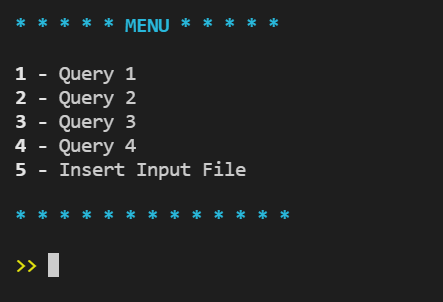
\includegraphics[scale=0.85]{images/menu}
	\captionof{figure}{Menu}
	\end{center}
	

\chapter{Codificação e Testes}  	% ---------------------------------------------------------- Codificação e Testes 

\section{Testes realizados e Resultados}
De seguida, são apresentados os testes e os respetivos resultados obtidos com as várias queries pedidas no enunciado.
\begin{itemize}
\item \textbf{Query 1}\par
Código não compilado:
\begin{verbatim}
int lados[4].
int i = 0.
int saoLados = 1.

main():
    repeat{
        lados[i] = read.
        i++.
    } until(i>3).
    if ((lados[1] equals lados[0]) and (lados[2] equals lados[0]) and (lados[3] equals lados[0])) {
        saoLados = 1.
    }
    else{
        saoLados = 0.
    }.
    print(saoLados).
end
\end{verbatim}
Código compilado:
\begin{verbatim}
pushn 4
pushi 0
pushi 1
start
repeat0:
pushgp
pushi 0
padd
pushg 4
read
atoi
storen
pushg 4
pushi 1
add
storeg 4
pushg 4
pushi 3
sup
jz repeat0
pushgp
pushi 0
padd
pushi 1
loadn
pushgp
pushi 0
padd
pushi 0
loadn
equal
pushgp
pushi 0
padd
pushi 2
loadn
pushgp
pushi 0
padd
pushi 0
loadn
equal
pushgp
pushi 0
padd
pushi 3
loadn
pushgp
pushi 0
padd
pushi 0
loadn
equal
mul
mul
jz if0
pushi 1
storeg 5
jump ifend0
if0:
pushi 0
storeg 5
ifend0:
stop
\end{verbatim}
\item \textbf{Query 2}\par
Código não compilado:
\begin{verbatim}
int n.
int menor.
int counter.
int aux.

main():
n = read.
repeat{
    if (counter equals 0) {menor = read.}
    else {
        aux = read.
        if (aux < menor) {menor = aux.}.
         }.
counter++.
}
until (counter moreEq n).
print menor.
end
\end{verbatim}
Código compilado:
\begin{verbatim}
pushi 0
pushi 0
pushi 0
pushi 0
start
read
atoi
storeg 0
repeat0:
pushg 2
pushi 0
equal
jz if1
read
atoi
storeg 1
jump ifend1
if1:
read
atoi
storeg 3
pushg 3
pushg 1
inf
jz if0
pushg 3
storeg 1
if0:
ifend1:
pushg 2
pushi 1
add
storeg 2
pushg 2
pushg 0
supeq
jz repeat0
pushg 1
writei
stop
\end{verbatim}
\item \textbf{Query 3}\par
Código não compilado:
\begin{verbatim}
int N.
int i.
int num.
int res.


main():
    print "Indique o nº de números a ler:\n".
    N = read.

    repeat{
        print "Indique um número:\n".
        num = read.
        if(res equals 0){
            res = res + num.
        }
        else {
            res = res * num.
        }.
        i++.
    }until(i moreEq N).

    print res.
end

\end{verbatim}
Código compilado:
\begin{verbatim}
pushi 0
pushi 0
pushi 0
pushi 0
start
pushs "Indique o nº de números a ler:\n"
writes
read
atoi
storeg 0
repeat0:
pushs "Indique um número:\n"
writes
read
atoi
storeg 2
pushg 3
pushi 0
equal
jz if0
pushg 3
pushg 2
add
storeg 3
jump ifend0
if0:
pushg 3
pushg 2
mul
storeg 3
ifend0:
pushg 1
pushi 1
add
storeg 1
pushg 1
pushg 0
supeq
jz repeat0
pushg 3
writei
stop
\end{verbatim}
\item \textbf{Query 4}\par
Código não compilado:
\begin{verbatim}
int v[5].
int N = 5.
int i.
int num.

main():
repeat{
    num = read.
    v[i] = num.
    i++.
}until(i equals N).

repeat{
    i--.
    print v[i].
}until(i equals 0).
end

\end{verbatim}
Código compilado:
\begin{verbatim}
pushn 5
pushi 5
pushi 0
pushi 0
start
repeat0:
read
atoi
storeg 7
pushgp
pushi 0
padd
pushg 6
pushg 7
storen
pushg 6
pushi 1
add
storeg 6
pushg 6
pushg 5
equal
jz repeat0
repeat1:
pushg 6
pushi 1
sub
storeg 6
pushgp
pushi 0
padd
pushg 6
loadn
writei
pushg 6
pushi 0
equal
jz repeat1
stop
\end{verbatim}

\end{itemize}
\newpage

\section{Problemas e Decisões}
Durante o desenvolvimento da GIC,o grupo decidiu utilizar recursividade à direita, no entanto, uma alternativa mais eficiente seria recorrer à recursividade à esquerda. A escolha da recursiviadade à direita deveu-se ao facto de esta ser mais fácil e intuitiva de implementar.
\vspace{3ex}
	  


\chapter{Conclusão} \label{concl}
A resolução deste projeto permitiu ao grupo consolidar toda a matéria lecionada ao longo das aulas teóricas e práticas relativa às gramáticas independentes do contexto e tradutoras. Além disto, permitiu aprofundar ainda mais o nosso conhecimento em Python.\par
Consideramos que realizamos o trabalho com sucesso, na medida em que respondemos a todos os requisitos pedidos no enunciado, obtendo os resultados bastante plausíveis.\par



\appendix % apendice
\chapter{Código do Programa}

\begin{verbatim}

import ply.yacc as yacc
from etelbina_lex import tokens


def p_Aplicacao(p):
    "Aplicacao : Declaracoes Content"
    global fwrite 
    fwrite.write(f"{p[1]}{p[2]}")

def p_Content(p):
    "Content : function Instrucoes end"
    p[0] = "start\n" + str(p[2]) + "stop\n"

def p_Declaracoes(p):
    " Declaracoes : Declaracao '.' Declaracoes"
    p[0] = p[1] + p[3]

def p_DeclaracoesEmpty(p):
    "Declaracoes : "
    p[0] = ""

def p_Declaracao(p):
    "Declaracao : int var"
    if p[2] in p.parser.variaveis:
        p[0] = f"err \"ERROR. Variavel ja declarada:\"\n"
        print(f"ERROR. Variável já declarada:'{p[2]}'")
        parser.success = False
    else:
        p.parser.variaveis[p[2]] = ["int",p.parser.sp]
        p[0]=("pushi 0\n")
        p.parser.sp+=1

def p_Declaracao_Array(p):
    "Declaracao : int var '[' num ']'"
    if p[2] in p.parser.variaveis:
        p[0] = f"err \"ERROR. Variavel ja declarada:\"\n"
        print(f"ERROR. Variável já declarada:'{p[2]}'")
        parser.success = False
    else:
        p[0]=(f"pushn {int(p[4])}\n")
        p.parser.variaveis[p[2]] = ["array",int(p[4]),p.parser.sp]
        p.parser.sp+=int(p[4])

def p_Declaracao_DoubleArray(p):
    "Declaracao : int var '[' num ']' '[' num ']'"
    if p[2] in p.parser.variaveis:
        p[0] = f"err \"ERROR. Variavel ja declarada:\"\n"
        print(f"ERROR. Variável já declarada:'{p[2]}'")
        parser.success = False
    else:
        p[0]=(f"pushn {(int(p[4])*int(p[7]))}\n")
        p.parser.variaveis[p[2]] = ["array",(int(p[4])*int(p[7])),int(p[4]),int(p[7]),p.parser.sp]
        p.parser.sp+=(int(p[4])*int(p[7]))


def p_Declaracao_atribuicao(p):
    "Declaracao : int var '=' NumNP"
    if p[2] in p.parser.variaveis:
        p[0] = f"err \"ERROR. Variavel ja declarada:\"\n"
        print(f"ERROR. Variável já declarada:'{p[2]}'")
        parser.success = False
    else:
        p.parser.variaveis[p[2]] = ["int",p.parser.sp]
        p[0]= p[4]
        p.parser.sp+=1

def p_Declaracao_Array_Atribuicao(p):
    "Declaracao : int var '[' num ']' '=' '{' Array '}'"
    if p[2] in p.parser.variaveis:
        p[0] = f"err \"ERROR. Variavel ja declarada:\"\n"
        print(f"ERROR. Variável já declarada:'{p[2]}'")
        parser.success = False
    else:
        p[0] = p[8]
        if p.parser.elemsCount == int(p[4]):
            p.parser.variaveis[p[2]] = ["array",int(p[4]),p.parser.sp]
            p.parser.sp+=int(p[4])
        else:
            p[0] = f"err \"ERROR. Elementos do array nao coincide com a declaracao\"\n"
            print(f"ERROR. Elementos do array nao coincide com a declaracao'{p[2]}'")
            parser.success = False
    p.parser.elemsCount = 0


def p_Declaracao_DoubleArray_Atribuicao(p):
    "Declaracao : int var '[' num ']' '[' num ']' '=' '{' DoubleArray '}'"
    if p[2] in p.parser.variaveis:
        p[0] = f"err \"ERROR. Variavel ja declarada:\"\n"
        print(f"ERROR. Variável já declarada:'{p[2]}'")
        parser.success = False
    else:
        p[0] = p[11]
        i = int(p[4])
        j = int(p[7])
        if (i==p.parser.elems2Count)and(j==p.parser.colCount)and(i*j==p.parser.elemsCount):
            p.parser.variaveis[p[2]] = ["array",i*j,i,j,p.parser.sp]
            p.parser.sp+=(i*j)
        else:
            p[0] = f"err \"ERROR. Elementos do array nao coincide com a declaracao\"\n"
            print(f"ERROR. Elementos do array nao coincide com a declaracao'{p[2]}'")
            parser.success = False
    p.parser.elemsCount = 0
    p.parser.elems2Count = 0
    p.parser.bool = 1


# ------------------ ARRAY/DOUBLE-ARRAY --------------------------

def p_DoubleArray(p):
    "DoubleArray : '{' Array '}' ElemsDArray"
    p[0] = p[2] + p[4]
    p.parser.elems2Count +=1

def p_ElemsDArray(p):
    "ElemsDArray : ',' '{' Array '}' ElemsDArray "
    p[0] = p[3] + p[5]
    p.parser.elems2Count +=1

def p_ElemsDArrayEmpty(p):
    "ElemsDArray : "
    p[0] = ""

def p_Array(p):
    "Array : NumNP Elems"
    p[0] = p[1] + p[2]
    p.parser.elemsCount +=1
    if(p.parser.bool==1):
        p.parser.colCount = p.parser.elemsCount
        p.parser.bool=0

def p_Elems(p):
    "Elems : ',' NumNP Elems"
    p[0] = p[2] + p[3]
    p.parser.elemsCount +=1

def p_Elems_Empty(p):
    "Elems : "
    p[0] = ""
    
    



# ----------------- INSTRUCOES ----------------------
def p_Instrucoes(p):
    "Instrucoes : Instrucao '.' Instrucoes"
    p[0] = p[1] + p[3]

def p_Instrucoes_Empty(p):
    "Instrucoes : "
    p[0] = ""

# ----------------- INSTRUÇÃO -------------------------

def p_Instrucao_Loop(p):
    "Instrucao : Loop"
    p[0] = p[1]

def p_Instrucao_Condition(p):
    "Instrucao : Condition"
    p[0]=(f"{p[1]}")


def p_Instrucao_Print(p):
    "Instrucao : Print"
    p[0]=(f"{p[1]}")
    

def p_Instrucao_Read(p):
    "Instrucao : VarArray '=' read "
    if(len(p[1])==3):
        p[0] =  p[1][0] + p[1][1] + (f"read\natoi\n") + "storen\n"
    else :
        p[0] = (f"read\natoi\n") + p[1][0]
        

def p_Instrucao_Expressao(p):
    "Instrucao : VarArray '=' Expressao"
    if(len(p[1])==3):
        p[0] = p[1][0] + p[1][1] + p[3] + p[1][2]
    else :
        p[0] = p[3] + p[1][0]

def p_Instrucao_MaisMais(p):
    "Instrucao : VarArray inc"
    if(len(p[1])==3):
        p[0] = p[1][0] + p[1][1] + p[1][0] + p[1][1] + "loadn\n" + "pushi 1\nadd\n" + p[1][2]
    else :
        p[0] = p[1][1] + "pushi 1\nadd\n" + p[1][0]


def p_Instrucao_MenosMenos(p):
    "Instrucao : VarArray dec"
    if(len(p[1])==3):
        p[0] = p[1][0] + p[1][1] + p[1][0] + p[1][1] + "loadn\n" + "pushi 1\nsub\n" + p[1][2]
    else :
        p[0] = p[1][1] + "pushi 1\nsub\n" + p[1][0]

# ----------------- LOOP ---------------------------
def p_Loop(p):
    "Loop : repeat '{' Instrucoes '}' until Verifica"
    p[0] = f"repeat{p.parser.loopCount}:\n{p[3]}{p[6]}jz repeat{p.parser.loopCount}\n"
    p.parser.loopCount +=1


#----------------IF ELSE------------------------

def p_Condition(p):
    "Condition : if Verifica '{' Instrucoes '}' "
    p[0] = f"{p[2]}jz if{p.parser.labelCount}\n{p[4]}if{p.parser.labelCount}:\n"
    p.parser.labelCount+=1
    

def p_Condition_else(p):
    "Condition : if Verifica '{' Instrucoes '}' else '{' Instrucoes	'}' "
    p[0] = f"{p[2]}jz if{p.parser.labelCount}\n{p[4]}jump ifend{parser.labelCount}\nif{p.parser.labelCount}:\n{p[8]}ifend{parser.labelCount}:\n"

    

#-------------------- VERIFICA ----------------------
def p_Verifica_cond(p):
    "Verifica : '(' Cond ')' "
    p[0] = p[2]

def p_Verifica_naocond(p):
    "Verifica : '!' '(' Cond ')' "
    p[0] = f"{p[3]}not\n"

def p_Verifica_And(p):
    "Verifica : Verifica and Verifica"
    p[0] = f"{p[1]}{p[3]}mul\n"

def p_Verifica_Or(p):
    "Verifica : Verifica or Verifica"
    p[0] = f"{p[1]}{p[3]}add\n{p[1]}{p[3]}mul\nsub\n"


# ----------------- COND ----------------------------
def p_Cond_Equals(p):
    "Cond : Expressao equals Expressao"
    p[0] = f"{p[1]}{p[3]}equal\n"

def p_Cond_LessEq(p):
    "Cond : Expressao lessEq Expressao"
    p[0] = f"{p[1]}{p[3]}infeq\n"

def p_Cond_MoreEq(p):
    "Cond : Expressao moreEq Expressao"
    p[0] = f"{p[1]}{p[3]}supeq\n"

def p_Cond_Menor(p):
    "Cond : Expressao '<' Expressao"
    p[0] = f"{p[1]}{p[3]}inf\n"

def p_Cond_Maior(p):
    "Cond : Expressao '>' Expressao"
    p[0] = f"{p[1]}{p[3]}sup\n"

def p_Cond_Verifica(p):
    "Cond : Verifica"
    p[0] = p[1]


#------------------- PRINT -----------------------------
def p_Print_VarArray(p):
    "Print : print VarArray"
    if(len(p[2])==3):
        p[0] = p[2][0]  + p[2][1] + "loadn\n" +"writei\n"
    else :
        p[0] = p[2][1] +"writei\n"


def p_Print_string(p):
    "Print : print string"
    p[0] = f"pushs {p[2]}\nwrites\n"



#------------------------ EXPRESSAO -------------------------

def p_Expressao_mais(p):
    "Expressao : Expressao '+' Termo"
    p[0] = p[1] + p[3] + "add\n"

def p_Expressao_menos(p):
    "Expressao : Expressao '-' Termo"
    p[0] = p[1] + p[3] + "sub\n"

def p_Expressao_Termo(p):
    "Expressao : Termo"
    p[0] = p[1]

def p_Termo_multi(p):
    "Termo : Termo '*' Fator"
    p[0] = p[1] + p[3] + "mul\n"
  
def p_Termo_div(p):
    "Termo : Termo '/' Fator"
    p[0] = p[1] + p[3] + "div\n"

def p_Termo_fator(p):
    "Termo : Fator"
    p[0] = p[1]
  
def p_Fator_VarN(p):
    "Fator : NumNP"
    p[0]=p[1]

def p_Fator_VarArray(p):
    "Fator : VarArray"
    if(len(p[1])==3):
        p[0] = p[1][0] + p[1][1] + "loadn\n"
    else :
        p[0] = p[1][1]

def p_Fator_expressao(p):
    "Fator : '(' Expressao ')' "
    p[0] = p[2]


def p_NumNP_NumNeg(p):
    "NumNP : numNeg"
    p[0] = f"pushi {p[1]}\n"

def p_NumNP_Num(p):
    "NumNP : num"
    p[0] = f"pushi {p[1]}\n"


def p_VarArray_array(p):
    "VarArray : var '[' Expressao ']'"
    if p[1] not in p.parser.variaveis:
        p[0] = f"err \"ERROR. Variavel nao declarada:\"\n"
        print(f"ERROR. Variavel nao declarada:'{p[1]}'")
        parser.success = False
    else:
        p[0] = (f"pushgp\npushi {p.parser.variaveis[p[1]][2]}\npadd\n" , p[3] , "storen\n")



def p_VarArray_double_array(p):
    "VarArray : var '[' Expressao ']' '[' Expressao ']'"
    if p[1] not in p.parser.variaveis:
        p[0] = f"err \"ERROR. Variavel nao declarada:\"\n"
        print(f"ERROR. Variavel nao declarada:'{p[1]}'")
        parser.success = False
    else:
        col = p.parser.variaveis[p[1]][3]
        p[0] = (f"pushgp\npushi {p.parser.variaveis[p[1]][4]}\npadd\n", p[3] + f"pushi {col}\n" + "mul\n" + p[6] + "add\n" , "storen\n")


def p_VarArray_var(p):
    "VarArray : var"
    if p[1] not in p.parser.variaveis:
        p[0] = f"err \"ERROR. Variavel nao declarada:\"\n"
        print(f"ERROR. Variavel nao declarada:'{p[1]}'")
        parser.success = False
    else:
        p[0] = (f"storeg {p.parser.variaveis[p[1]][1]}\n",f"pushg {p.parser.variaveis[p[1]][1]}\n")



def p_error(p):
    print('Erro sintático: ', p)
    parser.success = False


# Build the parser
parser = yacc.yacc()
parser.variaveis = {}
parser.sp = 0
parser.labelCount = 0
parser.loopCount = 0
parser.elemsCount = 0
parser.elems2Count = 0
parser.bool = 1


# Read line from input and parser it
import sys

def main():
    choice = '1'

    print("\n\033[1;36m* * * * * MENU * * * * *\033[00m\n")
    print("\033[;1m1 - \033[00mQuery 1")
    print("\033[;1m2 - \033[00mQuery 2")
    print("\033[;1m3 - \033[00mQuery 3")
    print("\033[;1m4 - \033[00mQuery 4")
    print("\033[;1m5 - \033[00mInsert Input File")

    print("\n\033[1;36m* * * * * * * * * * * * *\033[00m\n")
    choice = input ("\033[33m>> \033[00m")

    if choice == "5":
        menu_5()
    elif choice == "4":
        get_files("q4")
    elif choice == "3":
        get_files("q3")
    elif choice == "2":
        get_files("q2")
    elif choice == "1":
        get_files("q1")
    else:
        print("\033[1;31mInvalid Option!\n\033[00m")

def menu_5():
    try:
        print("Insert name of the input file: \n")
        fInput = input()
        fread = open("test_files/"+fInput, "r")
        print("Insert name of the output file: \n")
        fOutput = input()
        global fwrite 
        fwrite= open("test_files/"+fOutput,"w+")
        content = fread.read()
        res = parser.parse(content)
        print(parser.variaveis)
        fwrite.close()
    except:
        print('\033[1;31mError. Input file does not exist.\n\033[00m')
    

def get_files(file):
    fread = open("test_files/"+file+"_code.txt", "r")
    global fwrite 
    fwrite = open("test_files/"+file+"_vm.txt","w+")
    content = fread.read()
    res = parser.parse(content)
    print(parser.variaveis)
    fwrite.close()

fwrite = ""
main()
\end{verbatim}

\end{document} 